% Options for packages loaded elsewhere
\PassOptionsToPackage{unicode}{hyperref}
\PassOptionsToPackage{hyphens}{url}
%
\documentclass[
  american,
  man]{apa7}
\usepackage{amsmath,amssymb}
\usepackage{lmodern}
\usepackage{ifxetex,ifluatex}
\ifnum 0\ifxetex 1\fi\ifluatex 1\fi=0 % if pdftex
  \usepackage[T1]{fontenc}
  \usepackage[utf8]{inputenc}
  \usepackage{textcomp} % provide euro and other symbols
\else % if luatex or xetex
  \usepackage{unicode-math}
  \defaultfontfeatures{Scale=MatchLowercase}
  \defaultfontfeatures[\rmfamily]{Ligatures=TeX,Scale=1}
\fi
% Use upquote if available, for straight quotes in verbatim environments
\IfFileExists{upquote.sty}{\usepackage{upquote}}{}
\IfFileExists{microtype.sty}{% use microtype if available
  \usepackage[]{microtype}
  \UseMicrotypeSet[protrusion]{basicmath} % disable protrusion for tt fonts
}{}
\makeatletter
\@ifundefined{KOMAClassName}{% if non-KOMA class
  \IfFileExists{parskip.sty}{%
    \usepackage{parskip}
  }{% else
    \setlength{\parindent}{0pt}
    \setlength{\parskip}{6pt plus 2pt minus 1pt}}
}{% if KOMA class
  \KOMAoptions{parskip=half}}
\makeatother
\usepackage{xcolor}
\IfFileExists{xurl.sty}{\usepackage{xurl}}{} % add URL line breaks if available
\IfFileExists{bookmark.sty}{\usepackage{bookmark}}{\usepackage{hyperref}}
\hypersetup{
  pdftitle={Study 6},
  pdfauthor={Blinded1, Blinded2, Blinded1, \& Blinded1},
  pdflang={en-US},
  pdfkeywords={keywords},
  hidelinks,
  pdfcreator={LaTeX via pandoc}}
\urlstyle{same} % disable monospaced font for URLs
\usepackage{graphicx}
\makeatletter
\def\maxwidth{\ifdim\Gin@nat@width>\linewidth\linewidth\else\Gin@nat@width\fi}
\def\maxheight{\ifdim\Gin@nat@height>\textheight\textheight\else\Gin@nat@height\fi}
\makeatother
% Scale images if necessary, so that they will not overflow the page
% margins by default, and it is still possible to overwrite the defaults
% using explicit options in \includegraphics[width, height, ...]{}
\setkeys{Gin}{width=\maxwidth,height=\maxheight,keepaspectratio}
% Set default figure placement to htbp
\makeatletter
\def\fps@figure{htbp}
\makeatother
\setlength{\emergencystretch}{3em} % prevent overfull lines
\providecommand{\tightlist}{%
  \setlength{\itemsep}{0pt}\setlength{\parskip}{0pt}}
\setcounter{secnumdepth}{-\maxdimen} % remove section numbering
% Make \paragraph and \subparagraph free-standing
\ifx\paragraph\undefined\else
  \let\oldparagraph\paragraph
  \renewcommand{\paragraph}[1]{\oldparagraph{#1}\mbox{}}
\fi
\ifx\subparagraph\undefined\else
  \let\oldsubparagraph\subparagraph
  \renewcommand{\subparagraph}[1]{\oldsubparagraph{#1}\mbox{}}
\fi
% Manuscript styling
\usepackage{upgreek}
\captionsetup{font=singlespacing,justification=justified}

% Table formatting
\usepackage{longtable}
\usepackage{lscape}
% \usepackage[counterclockwise]{rotating}   % Landscape page setup for large tables
\usepackage{multirow}		% Table styling
\usepackage{tabularx}		% Control Column width
\usepackage[flushleft]{threeparttable}	% Allows for three part tables with a specified notes section
\usepackage{threeparttablex}            % Lets threeparttable work with longtable

% Create new environments so endfloat can handle them
% \newenvironment{ltable}
%   {\begin{landscape}\begin{center}\begin{threeparttable}}
%   {\end{threeparttable}\end{center}\end{landscape}}
\newenvironment{lltable}{\begin{landscape}\begin{center}\begin{ThreePartTable}}{\end{ThreePartTable}\end{center}\end{landscape}}

% Enables adjusting longtable caption width to table width
% Solution found at http://golatex.de/longtable-mit-caption-so-breit-wie-die-tabelle-t15767.html
\makeatletter
\newcommand\LastLTentrywidth{1em}
\newlength\longtablewidth
\setlength{\longtablewidth}{1in}
\newcommand{\getlongtablewidth}{\begingroup \ifcsname LT@\roman{LT@tables}\endcsname \global\longtablewidth=0pt \renewcommand{\LT@entry}[2]{\global\advance\longtablewidth by ##2\relax\gdef\LastLTentrywidth{##2}}\@nameuse{LT@\roman{LT@tables}} \fi \endgroup}

% \setlength{\parindent}{0.5in}
% \setlength{\parskip}{0pt plus 0pt minus 0pt}

% Overwrite redefinition of paragraph and subparagraph by the default LaTeX template
% See https://github.com/crsh/papaja/issues/292
\makeatletter
\renewcommand{\paragraph}{\@startsection{paragraph}{4}{\parindent}%
  {0\baselineskip \@plus 0.2ex \@minus 0.2ex}%
  {-1em}%
  {\normalfont\normalsize\bfseries\itshape\typesectitle}}

\renewcommand{\subparagraph}[1]{\@startsection{subparagraph}{5}{1em}%
  {0\baselineskip \@plus 0.2ex \@minus 0.2ex}%
  {-\z@\relax}%
  {\normalfont\normalsize\itshape\hspace{\parindent}{#1}\textit{\addperi}}{\relax}}
\makeatother

% \usepackage{etoolbox}
\makeatletter
\patchcmd{\HyOrg@maketitle}
  {\section{\normalfont\normalsize\abstractname}}
  {\section*{\normalfont\normalsize\abstractname}}
  {}{\typeout{Failed to patch abstract.}}
\patchcmd{\HyOrg@maketitle}
  {\section{\protect\normalfont{\@title}}}
  {\section*{\protect\normalfont{\@title}}}
  {}{\typeout{Failed to patch title.}}
\makeatother
\keywords{keywords\newline\indent Word count: TBC}
\DeclareDelayedFloatFlavor{ThreePartTable}{table}
\DeclareDelayedFloatFlavor{lltable}{table}
\DeclareDelayedFloatFlavor*{longtable}{table}
\makeatletter
\renewcommand{\efloat@iwrite}[1]{\immediate\expandafter\protected@write\csname efloat@post#1\endcsname{}}
\makeatother
\usepackage{csquotes}
\usepackage[titles]{tocloft}
\cftpagenumbersoff{figure}
\renewcommand{\cftfigpresnum}{\itshape\figurename\enspace}
\renewcommand{\cftfigaftersnum}{.\space}
\setlength{\cftfigindent}{0pt}
\setlength{\cftafterloftitleskip}{0pt}
\settowidth{\cftfignumwidth}{Figure 10.\qquad}
\cftpagenumbersoff{table}
\renewcommand{\cfttabpresnum}{\itshape\tablename\enspace}
\renewcommand{\cfttabaftersnum}{.\space}
\setlength{\cfttabindent}{0pt}
\setlength{\cftafterloftitleskip}{0pt}
\settowidth{\cfttabnumwidth}{Table 10.\qquad}
\raggedbottom
\ifxetex
  % Load polyglossia as late as possible: uses bidi with RTL langages (e.g. Hebrew, Arabic)
  \usepackage{polyglossia}
  \setmainlanguage[variant=american]{english}
\else
  \usepackage[main=american]{babel}
% get rid of language-specific shorthands (see #6817):
\let\LanguageShortHands\languageshorthands
\def\languageshorthands#1{}
\fi
\ifluatex
  \usepackage{selnolig}  % disable illegal ligatures
\fi
\newlength{\cslhangindent}
\setlength{\cslhangindent}{1.5em}
\newlength{\csllabelwidth}
\setlength{\csllabelwidth}{3em}
\newenvironment{CSLReferences}[2] % #1 hanging-ident, #2 entry spacing
 {% don't indent paragraphs
  \setlength{\parindent}{0pt}
  % turn on hanging indent if param 1 is 1
  \ifodd #1 \everypar{\setlength{\hangindent}{\cslhangindent}}\ignorespaces\fi
  % set entry spacing
  \ifnum #2 > 0
  \setlength{\parskip}{#2\baselineskip}
  \fi
 }%
 {}
\usepackage{calc}
\newcommand{\CSLBlock}[1]{#1\hfill\break}
\newcommand{\CSLLeftMargin}[1]{\parbox[t]{\csllabelwidth}{#1}}
\newcommand{\CSLRightInline}[1]{\parbox[t]{\linewidth - \csllabelwidth}{#1}\break}
\newcommand{\CSLIndent}[1]{\hspace{\cslhangindent}#1}

\title{Study 6}
\author{Blinded\textsuperscript{1}, Blinded\textsuperscript{2}, Blinded\textsuperscript{1}, \& Blinded\textsuperscript{1}}
\date{}


\shorttitle{Cognitive Load and Moral Dumbfounding}

\authornote{

Correspondence concerning this article should be addressed to Blinded, Blinded. E-mail: Blinded

}

\affiliation{\vspace{0.5cm}\textsuperscript{1} Blinded\\\textsuperscript{2} Blinded}

\abstract{
Six studies etc.
}



\begin{document}
\maketitle

\hypertarget{study-6---pre-registered-replication}{%
\section{Study 6 - Pre-registered Replication}\label{study-6---pre-registered-replication}}

In response to the mixed findings in Studies 1-5, the aim of Study 6 was to test if cognitive load influences participants' ability to justify their judgments in high-powered, large sample study. Study 6 was pre-registered (see \url{https://aspredicted.org/XZP_UHW}).

\hypertarget{study-6-method}{%
\subsection{Study 6: Method}\label{study-6-method}}

\hypertarget{study-6-participants-and-design}{%
\subsubsection{Study 6: Participants and design}\label{study-6-participants-and-design}}

Study 6 was a between subjects design. The dependent variable was rates of providing reasons/dumbfounding (measured using to the critical slide as in previous studies). The primary independent variable was cognitive load with two levels: present and absent. To manipulate cognitive load, a stream of numbers scrolled across the screen above the question text, and participants were required to pay attention to how many times they saw a given number. Scenario served as a secondary independent variable, we used four scenarios: \emph{Julie and Mark (Incest)}, \emph{Jennifer (Cannibal)}, \emph{Trolley}, \emph{Heinz}.

A total sample of 1899 participants (984 female, 876 male, 17 non-binary, 1 other, 5 prefer not to say; \emph{M}\textsubscript{age} = 43.22, min = 18, max = 84, \emph{SD} = 15.85) started the survey. Participants in this sample were recruited from Prolific (\emph{n\textsubscript{UK}} = 963, \emph{n\textsubscript{US}} = 936).

Participants who failed both manipulation checks (\emph{n} = 7) or who had missing data for the measures of interest were removed, leaving a total sample of 1686 participants (867 female, 799 male, 14 non-binary, 1 other, 5 prefer not to say; \emph{M}\textsubscript{age} = 43.81, min = 18, max = 83, \emph{SD} = 15.76), \emph{n\textsubscript{UK}} = 842, \emph{n\textsubscript{US}} = 844.

\hypertarget{study-6-procedure-and-materials}{%
\subsubsection{Study 6: Procedure and materials}\label{study-6-procedure-and-materials}}

Data were collected using an online questionnaire developed with jsPsych and distributed with cognition.run. Participants were presented with one of four moral scenarios (\emph{Julie and Mark}, \emph{Jennifer}, \emph{Trolley}, \emph{Heinz}, see supplementary materials for full wording), previously used in studies of moral dumbfounding (McHugh et al., 2017). The sequence of responses was similar to previous studies, but with content of questions and counter arguments updated to match the relevant scenarios (see supplementary materials).

To manipulate cognitive load manipulation in Study 6, drawing on Greene, Morelli, Lowenberg, Nystrom, and Cohen (2008) we included a video stream of numbers scrolling above the question text. The video was wide enough to display 3 numbers at a time, and the numbers scrolled past at a speed of 2 numbers per second. Participants were asked to attend to and report (on a subsequent page) how many times a particular number appeared in the stream, while answering the target question. Following an initial training task, the video was presented while participants made their initial judgments, while they responded to the critical slide, and while they were providing their revised judgments.

Two attention check tasks were included for all participants, these included a brief paragraph of text where instructions for the correct response were embedded within the text. The wording of the text was misleading such that if participants skimmed or only read some of the text they would likely provide an incorrect response. In order to keep the survey short to facilitate the recruiting of a large sample, we did not record Need for Cognition in Study 6.

Participants clicked on the survey link and were randomly assigned to either the experimental condition or the control condition, within which they were randomly presented with one of the four scenarios. The study was complete within 5 minutes.

\hypertarget{study-6-results}{%
\subsection{Study 6: Results}\label{study-6-results}}

One thousand three hundred sixty-five participants (80.96\%) rated the behavior described as wrong initially, and one thousand three hundred forty three participants (79.66\%) rated the behavior as wrong at the end of the task. Initial ratings (\emph{M} = 2.26, \emph{SD} = 1.63) were significantly more severe than revised ratings (\emph{M} = 2.34, \emph{SD} = 1.66), \emph{t}(1685) = -2.69, \emph{p} = .007; \emph{d} = 0.07. Inspection of the binned judgments revealed that two hundred (11.86\%) participants changed the valence of their judgments, breakdown of the changes in judgments is in Table XX (full sample) and Table XX (by scenario) in the supplementary materials.

A 2 \(\times\) 2 factorial ANOVA revealed significant differences in initial judgments depending on both condition \emph{F}(1, 1678) = 26.65, \emph{p} \textless{} .001, partial \(\eta\)\textsuperscript{2} = .016, and scenario \emph{F}(3, 1678) = 69.30, \emph{p} \textless{} .001, partial \(\eta\)\textsuperscript{2} = .110. Participants under cognitive load were significantly (\emph{p} \textless{} .001) less harsh in their judgments (\emph{M} = 2.46, \emph{SD} = 1.75) than those in the control condition (\emph{M} = 2.07, \emph{SD} = 1.49). Participants rated \emph{Jennifer} as the most wrong (\emph{M} = 1.53, \emph{SD} = 1.13), followed by \emph{Julie and Mark} (\emph{M} = 2.05, \emph{SD} = 1.65, \emph{p} \textless{} .001), then \emph{Heinz} (\emph{M} = 2.49, \emph{SD} = 1.65, \emph{p} \textless{} .001), with \emph{Trolley} receiving the least severe judgment (\emph{M} = 2.98, \emph{SD} = 1.69, \emph{p} \textless{} .001). There was no significant condition \(\times\) scenario interaction \emph{F}(3, 1678) = 0.46, \emph{p} = .708, partial \(\eta\)\textsuperscript{2} \textless{} .001.

A 2 \(\times\) 2 factorial ANOVA revealed significant differences in revised judgments depending on both condition \emph{F}(1, 1678) = 12.82, \emph{p} \textless{} .001, partial \(\eta\)\textsuperscript{2} = .008, and scenario \emph{F}(3, 1678) = 80.69, \emph{p} \textless{} .001, partial \(\eta\)\textsuperscript{2} = .126. Participants under cognitive load were significantly (\emph{p} \textless{} .001) less harsh in their judgments (\emph{M} = 2.47, \emph{SD} = 1.71) than those in the control condition (\emph{M} = 2.20, \emph{SD} = 1.59). Participants rated \emph{Jennifer} as the most wrong (\emph{M} = 1.54, \emph{SD} = 1.12), followed by \emph{Julie and Mark} (\emph{M} = 2.15, \emph{SD} = 1.73, \emph{p} \textless{} .001), then \emph{Heinz} (\emph{M} = 2.52, \emph{SD} = 1.58, \emph{p} = .003), with \emph{Trolley} receiving the least severe judgment (\emph{M} = 3.14, \emph{SD} = 1.72, \emph{p} \textless{} .001). There was no significant condition \(\times\) scenario interaction \emph{F}(3, 1678) = 1.34, \emph{p} = .260, partial \(\eta\)\textsuperscript{2} = .002.

Dumbfounding was recorded using the critical slides, participants who selected the admission of not having reasons on the critical slide were identified as dumbfounded. Four hundred and seventeen participants (24.73\%) selected ``It's wrong but I can't think of a reason.'' One thousand and thirty-two participants (61.21\%) selected ``It's wrong and I can provide a valid reason''; and two hundred and thirty-seven participants (14.06\%) selected ``There is nothing wrong.''

A chi-squared test for independence revealed a significant association between experimental condition and response to the critical slide, \(\chi\)\textsuperscript{2}(2, \emph{N} = 1686) = 25.48, \emph{p} \textless{} .001, \emph{V} = 0.12, the observed power was 0.997. As predicted, under cognitive load fewer participants (458; 55.45\%) provided reasons than in the control condition (574; 66.74\%), and more participants (245; 29.66\%) selected ``It's wrong but I can't think of a reason.'' than in the control group (172; 20\%). The responses to the critical slide for the experimental group (\emph{N} = 826) and the control group (\emph{N} = 860) are displayed in Figure~\ref{fig:S6ch5S6fig1criticalconditionb}. The observed counts, expected counts and standardised residuals are displayed in Table~\ref{tab:S6tab1dumb}.

\newpage

\begin{figure}
\centering
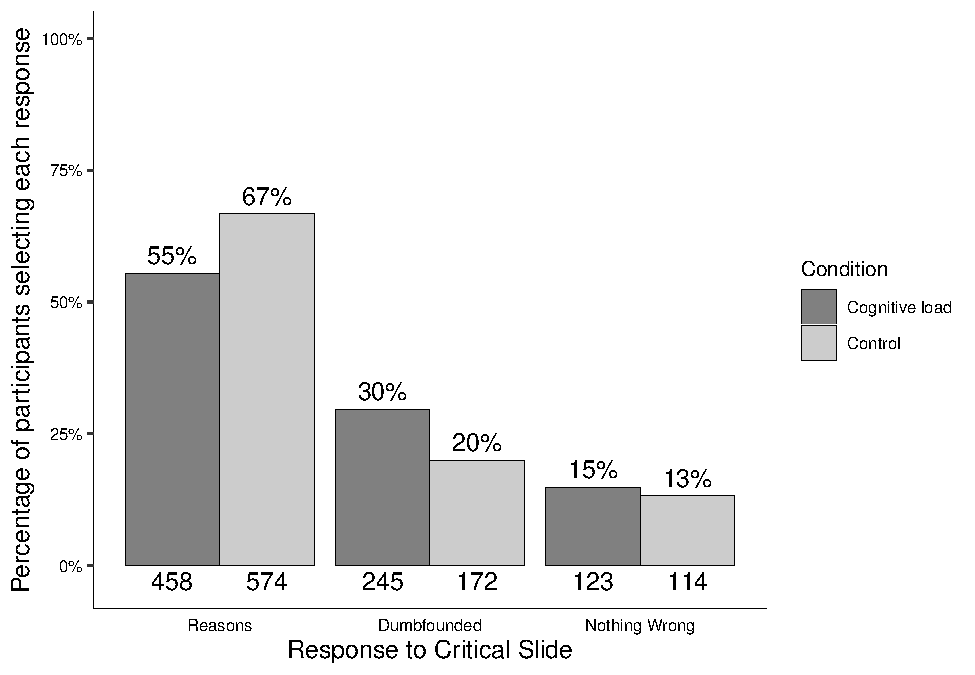
\includegraphics{Study_6_files/figure-latex/S6ch5S6fig1criticalconditionb-1.pdf}
\caption{\label{fig:S6ch5S6fig1criticalconditionb}Study 6: Responses to critical slide depending on cognitive load}
\end{figure}

\begin{table}[tbp]

\begin{center}
\begin{threeparttable}

\caption{\label{tab:S6tab1dumb}Study 6 – Observed counts, expected counts, and standardised residuals for each response to the critical slide depending on cognitive load (full sample)}

\begin{tabular}{llcc}
\toprule
 & \multicolumn{1}{c}{} & \multicolumn{1}{c}{Cognitive Load} & \multicolumn{1}{c}{Control}\\
\midrule
Observed count & Reasons & 458 & 574\\
 & Dumbfounded & 245 & 172\\
 & Nothing Wrong & 123 & 114\\
Expected count & Reasons & 505.59 & 526.41\\
 & Dumbfounded & 204.3 & 212.7\\
 & Nothing Wrong & 116.11 & 120.89\\
Standardised residuals & Reasons & -4.76** & 4.76**\\
 & Dumbfounded & 4.6** & -4.6**\\
 & Nothing Wrong & 0.97 & -0.97\\
\bottomrule
\addlinespace
\end{tabular}

\begin{tablenotes}[para]
\normalsize{\textit{Note.} * = sig. at \emph{p} < .05; ** = sig. at \emph{p} < .001}
\end{tablenotes}

\end{threeparttable}
\end{center}

\end{table}

\newpage

This pattern was observed for all scenarios individually with the exception of \emph{Julie and Mark}, which showed no association between experimental condition and cognitive load, \(\chi\)\textsuperscript{2}(2, \emph{N} = 418) = 0.49, \emph{p} = .783, \emph{V} = 0.25, power = 0.601. The association was significant for \emph{Jennifer} \(\chi\)\textsuperscript{2}(2, \emph{N} = 418) = 17.33, \emph{p} \textless{} .001, \emph{V} = 0.24, power = 0.623, \emph{Trolley} \(\chi\)\textsuperscript{2}(2, \emph{N} = 418) = 10.95, \emph{p} = .004, \emph{V} = 0.25, power = 0.614, and Heinz, \(\chi\)\textsuperscript{2}(2, \emph{N} = 418) = 7.16, \emph{p} = .028, \emph{V} = 0.25, power = 0.608, see Figure~\ref{fig:S6ch5S6fig2criticalconditionb}. Supplementary Tables XX-XX show the direction of the effect for each scenario. Under cognitive load, fewer participants provided reasons and more participants provided a dumbfounded response for \emph{Jennifer}, \emph{Trolley}, and \emph{Heinz}

\begin{figure}
\centering
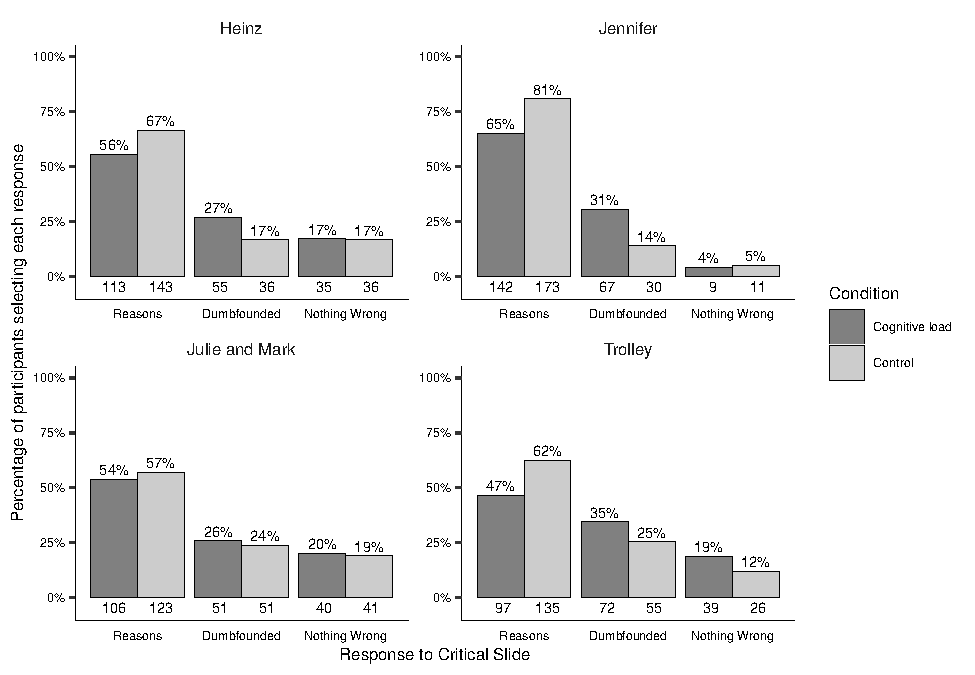
\includegraphics{Study_6_files/figure-latex/S6ch5S6fig2criticalconditionb-1.pdf}
\caption{\label{fig:S6ch5S6fig2criticalconditionb}Study 6: Responses to critical slide and for the experimental group and the control group for each scenario}
\end{figure}

A chi-squared test for independence revealed a significant association between scenario and response to the critical slide, \(\chi\)\textsuperscript{2}(6, \emph{N} = 1686) = 61.34, \emph{p} \textless{} .001, \emph{V} = 0.19, the observed power was 1. Participants were significantly more likely to select ``There is nothing wrong'' for \emph{Julie and Mark} (\emph{p} = .002), more likely to provide reasons (\emph{p} = .002) and less likely to select ``There is nothing wrong'' (\emph{p} \textless{} .001) for Jennifer, and more likely to be dumbfounded by \emph{Trolley} (\emph{p} = .031).

A multinomial logistic regression was conducted to test the effects of cognitive load and scenario on dumbfounded responding. Overall the model was significant, \(\chi\)\textsuperscript{2}(8, \emph{N} = 1686) = 95.9, \emph{p} \textless{} .001, and explained between 6.07\% (Cox and Snell R square) and 7.22\% (Nadelkerke R squared) of the variance in responses to the critical slide, the observed power was 1. Participants in the control condition were significantly less likely to provide a dumbfounded response than to provide reasons, Wald = 25.04, \emph{p} \textless{} .001, \emph{OR} = 0.55, 95\% CI {[}0.44, 0.70{]}, in addition, participants in the control condition were also signifcantly less likely to select ``There is nothing wrong,'' than to provide reasons, Wald = 5.23, \emph{p} = .022, \emph{OR} = 0.71, 95\% CI {[}0.54, 0.95{]}. For \emph{Jennifer}, participants were significantly less likely to select ``There is nothing wrong'' than to provide a reason, Wald = 30.87, \emph{p} \textless{} .001, \emph{OR} = 0.23, 95\% CI {[}0.13, 0.38{]}; while for \emph{Trolley} participants were significantly more likely to present as dumbfounded than to provide a reason, Wald = 6.89, \emph{p} = .009, \emph{OR} = 1.55, 95\% CI {[}1.12, 2.14{]}.

\hypertarget{refs}{}
\begin{CSLReferences}{1}{0}
\leavevmode\hypertarget{ref-greene_cognitive_2008}{}%
Greene, J. D., Morelli, S. A., Lowenberg, K., Nystrom, L. E., \& Cohen, J. D. (2008). Cognitive load selectively interferes with utilitarian moral judgment. \emph{Cognition}, \emph{107}(3), 1144--1154. \url{https://doi.org/10.1016/j.cognition.2007.11.004}

\leavevmode\hypertarget{ref-mchugh_searching_2017a}{}%
McHugh, C., McGann, M., Igou, E. R., \& Kinsella, E. L. (2017). Searching for {Moral Dumbfounding}: Identifying {Measurable Indicators} of {Moral Dumbfounding}. \emph{Collabra: Psychology}, \emph{3}(1), 1--24. \url{https://doi.org/10.1525/collabra.79}

\end{CSLReferences}


\clearpage
\renewcommand{\listfigurename}{Figure captions}

\clearpage
\renewcommand{\listtablename}{Table captions}


\end{document}
